Так как это вспомогательное приложение, для простоты разработки не будем создавать для него графический интерфейс. 

Задача состоит в создании приложения, которое ожидает подключения и при появлении такового создает новое tcp соединение и принимает информацию, так же приложение должно проверять статус соединения и при его разрыве удалять созданные сокеты для освобождения портов. Данный механизм в дальнейшем будет использоваться и на сервере.

Задачей управления соединениями занимается объект типа QTcpServer. Данный класс порождает объекты, которые, прослушивает порт и испускает сигналы при появлении запроса на соединение.

Создадим класс TestServ. Прототип класса представлен ниже.

\begin{lstlisting}
class TestServ : public QObject
{
    Q_OBJECT
public:
    explicit TestServ(QObject *parent = 0);
    ~TestServ();

    void initServ(const int &port);

private:
    QTcpServer *srv;
    QMap<QString, ClientSock*> users;
signals:

public slots:
    void newConnection();
    void connectClosed(QString name);
};
\end{lstlisting}

В конструкторе и диструктора класса инициилизируется объект srv, так же в конструкторе связывается сигнал объекта srv newConnection со слотом данного класса newConnection.

Метод initServ указывает объекту srv какой порт необходимо прослушивать, и выводит в консоль информацию о том, успешно ли прошел запуск сервера.

QMap<QString, ClientSock*> users - это контейнер для хранения указателей на созданные в даный момент сокеты с присвоенными им именами.

Слот newConnection() отрабатывает при появлении нового запроса на соединение, здесь в консоль выводится сообщение о создании нового запроса и создается и инициализируется объект ClientSock*, после чего его сигнал scDisconnect(QString) связывается со слотом connectClosed(QString) и указатель помещается в QMap.

Слот connectClosed принимает на вход имя слота, производит поиск укзателя с данным именем, отдает команду уничтожить объект и удаляет запись о данном объекте из QMap.

Объект ClientSock это ранее созданный класс EmulSock с добавлением нескольких методов и сигналов. Прототип данного класса представлен ниже.

\begin{lstlisting}
class ClientSock : public QObject
{
    Q_OBJECT
public:
    explicit ClientSock(QObject *parent = 0);
    explicit ClientSock(QTcpSocket *sock, QObject *parent = 0);
    ~ClientSock();
    void initSc(const QString & addr, const int & port);
    void setName(const QString & name);
    QString getName();
    void sendData(QByteArray data);
    void timerEvent(QTimerEvent *event);
private:
    QTcpSocket * sc;
    QString m_qsScName;
signals:
    void scDisconnect(QString);
public slots:
    QByteArray getData();
};
\end{lstlisting}

В описании добавился конструктор, принимающий указатель на объект QTcpSocket, необходимый для создания объекта на основании данных, полученных от объекта srv.

Методы getName и setName необходиы для работы с атрибутом m\_qsScName, хранящую имя объекта.

Метод timerEvent отслеживает статус сокета sc, данный метод вызывается всякий раз при обнулении таймера, запускаемого при создании объекта типа ClientSock в констукторе. Данный метод проверяет статус сокета и при получении статуса ``отключен'' останавливате таймер, выводит сообщение о прекращении соединения и испускает сигнал что соединение закрыто, который обрабатывается объектом типа TestServ.

В функции main просто создаем объект типа TestServ, и указываем ему порт назначения, переданный первым аргументом при запуске программы. Пример работы с подключением одного клиента представлен на рисунку \ref{clientEmul:clientEmul}.

\begin{figure}[h!]
 \center{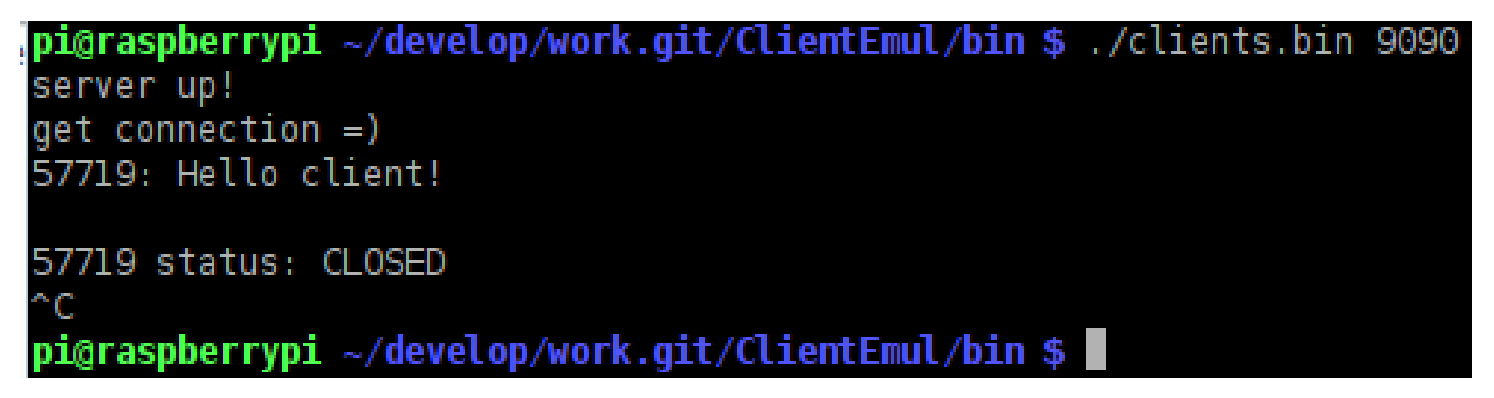
\includegraphics[width=0.7\linewidth]{clientEmul}}
 \caption{Демонстрация работы приложения}
 \label{clientEmul:clientEmul}
\end{figure}
